% questions.tex —— 2009 年·普通高等学校招生考试·辽宁卷·理科 · 题目内容片段（无答案）
% 由 tools/generate_projects.py 依来源总账自 2009/2009_数学真题_辽宁理_试题.md 生成，勿手改（改源 MD 后重跑）


状态：needs-review；依固定候选 PDF 两页（印刷页 537–538）逐题核验，图形已矢量重绘，正式构建与逐页验收见回执。源未标分值，不补分值。第 19 题原页印作「某人向一目射击 $4$ 次」，疑脱「标」字，照录原页并在解析中说明，另登记问题条目。第 22 题为三选一，原页只标「三选一」并以【A】【B】【C】分列三题，本转录照录，不补写作答规则。

\gkpart{一、选择题}

\begin{question}
\gkti{1}已知集合 $M=\{x\mid -3<x\leqslant5\}$，$N=\{x\mid -5<x<5\}$，则 $M\cap N=$（　）

（A）$\{x\mid -5<x<5\}$

（B）$\{x\mid -3<x<5\}$

（C）$\{x\mid -5<x\leqslant5\}$

（D）$\{x\mid -3<x\leqslant5\}$

\end{question}
\begin{question}
\gkti{2}已知复数 $z=1-2\mathrm i$，那么 $\frac1z=$（　）

（A）$\frac{\sqrt5}{5}+\frac{2\sqrt5}{5}\mathrm i$

（B）$\frac{\sqrt5}{5}-\frac{2\sqrt5}{5}\mathrm i$

（C）$\frac15+\frac25\mathrm i$

（D）$\frac15-\frac25\mathrm i$

\end{question}
\begin{question}
\gkti{3}平面向量 $\boldsymbol a$ 与 $\boldsymbol b$ 的夹角为 $60^\circ$，$\boldsymbol a=(2,0)$，$|\boldsymbol b|=1$，则 $|\boldsymbol a+2\boldsymbol b|=$（　）

（A）$\sqrt3$

（B）$2\sqrt3$

（C）$4$

（D）$12$

\end{question}
\begin{question}
\gkti{4}已知圆 $C$ 与直线 $x-y=0$ 及 $x-y-4=0$ 都相切，圆心在直线 $x+y=0$ 上，则圆 $C$ 的方程为（　）

（A）$(x+1)^2+(y-1)^2=2$

（B）$(x-1)^2+(y+1)^2=2$

（C）$(x-1)^2+(y-1)^2=2$

（D）$(x+1)^2+(y+1)^2=2$

\end{question}
\begin{question}
\gkti{5}从 $5$ 名男医生、$4$ 名女医生中选 $3$ 名医生组成一个医疗小分队，要求其中男、女医生都有，则不同的组队方案共有（　）

（A）$70$ 种

（B）$80$ 种

（C）$100$ 种

（D）$140$ 种

\end{question}
\begin{question}
\gkti{6}设等比数列 $\{a_n\}$ 的前 $n$ 项和为 $S_n$，若 $\frac{S_6}{S_3}=3$，则 $\frac{S_9}{S_6}=$（　）

（A）$2$

（B）$\frac73$

（C）$\frac83$

（D）$3$

\end{question}
\begin{question}
\gkti{7}曲线 $y=\frac{x}{x-2}$ 在点 $(1,-1)$ 处的切线方程为（　）

（A）$y=x-2$

（B）$y=-3x+2$

（C）$y=2x-3$

（D）$y=-2x+1$

\Needspace{0.4\textheight}
\end{question}
\begin{question}
\gkti{8}已知函数 $f(x)=A\cos(\omega x+\varphi)$ 的图象如图所示，$f\left(\frac{\pi}{2}\right)=-\frac23$，则 $f(0)=$（　）

（A）$-\frac23$

（B）$\frac23$

（C）$-\frac12$

（D）$\frac12$
\nopagebreak[4]
\begin{center}% 2009 年辽宁卷理科第 8 题：f(x)=Acos(ωx+φ) 的图象。
% 来源 PDF：普通高考/2009/2009辽宁理.pdf，SHA256 5ae9708acfe7def5bddd60a34d1474cfa2e2c20a39d130255e0e4393093accad
% 原页：第 1 页（A3 三栏）第 1 栏下部，印刷页 537。
% 重绘依据：曲线在 x=7π/12 与 x=11π/12 处与 x 轴相交，两零点之间为正值峰；
%   故半周期为 π/3、ω=3。又 x=π/2 处函数值为 −2/3（虚线标出），由此定出振幅，
%   进而 f(0)=2/3。原图只画峰附近一段，y 轴在左侧。
\begin{tikzpicture}[scale=1.15, semithick, >=Stealth,
  every node/.style={inner sep=1.5pt, font=\small}]
  \draw[->] (-0.55,0) -- (3.35,0) node[right] {$x$};
  \draw[->] (0,-1.35) -- (0,1.32) node[above] {$y$};
  \node[below left] at (0,0) {$O$};
  \draw[domain=1.22:3.12, samples=240, smooth, thick]
    plot (\x,{0.9428*sin(deg(3*(\x-1.8326)))});
  \draw[densely dashed] (0,-0.6667) -- (1.5708,-0.6667);
  \draw[densely dashed] (1.5708,-0.6667) -- (1.5708,0);
  \draw (1.8326,0.09) -- (1.8326,-0.09);
  \draw (2.8798,0.09) -- (2.8798,-0.09);
  \node[left] at (-0.06,-0.6667) {$-\frac23$};
  \node[above] at (1.5708,0.04) {$\frac{\pi}{2}$};
  \node[below] at (1.8326,-0.72) {$\frac{7\pi}{12}$};
  \node[below] at (2.8798,-0.72) {$\frac{11\pi}{12}$};
\end{tikzpicture}
\end{center}
\nopagebreak[4]
\end{question}
\begin{question}
\gkti{9}已知偶函数 $f(x)$ 在区间 $[0,+\infty)$ 单调增加，则满足 $f(2x-1)<f\left(\frac13\right)$ 的 $x$ 取值范围是（　）

（A）$\left(\frac13,\frac23\right)$

（B）$\left[\frac13,\frac23\right)$

（C）$\left(\frac12,\frac23\right)$

（D）$\left[\frac12,\frac23\right)$

\Needspace{0.4\textheight}
\end{question}
\begin{question}
\gkti{10}某店一个月的收入和支出总共记录了 $N$ 个数据 $a_1,a_2,\cdots,a_N$，其中收入记为正数，支出记为负数．该店用下边的程序框图计算月总收入 $S$ 和月净盈利 $V$，那么在图中空白的判断框和处理框中，应分别填入下列四个选项中的（　）

（A）$A>0$，$V=S-T$

（B）$A<0$，$V=S-T$

（C）$A>0$，$V=S+T$

（D）$A<0$，$V=S+T$
\nopagebreak[4]
\begin{center}% 2009 年辽宁卷理科第 10 题：计算月总收入 S 与月净盈利 V 的程序框图。
% 来源 PDF：普通高考/2009/2009辽宁理.pdf，SHA256 5ae9708acfe7def5bddd60a34d1474cfa2e2c20a39d130255e0e4393093accad
% 原页：第 1 页（A3 三栏）第 2 栏上部，印刷页 537。
% 重绘依据：开始 → 输入 N,a1,...,aN → k=1,S=0,T=0 → A=ak → 判断框（原页空白）：
%   否（左）T=T+A，是（右）S=S+A；两路汇合后判断 k<N：是（右）k=k+1 回到 A=ak，
%   否（下）输出 S,V → 结束。判断框内的条件在原页留空，由选项填入。
\begin{tikzpicture}[scale=0.82, semithick, >=Stealth,
  every node/.style={inner sep=3pt, font=\small}]
  \node (start) at (0,0) [draw, rounded corners=4pt, minimum width=2.1cm, minimum height=0.6cm] {开始};
  \node (input) at (0,-1.3) [draw, trapezium, trapezium left angle=75, trapezium right angle=105,
    minimum width=4.9cm, minimum height=0.72cm] {输入 $N,\,a_1,\,a_2,\,\cdots,\,a_N$};
  \node (init) at (0,-2.75) [draw, minimum width=4.0cm, minimum height=0.7cm] {$k=1,\ S=0,\ T=0$};
  \node (ak) at (0,-4.05) [draw, minimum width=1.75cm, minimum height=0.62cm] {$A=a_k$};
  \node (cond) at (0,-5.55) [draw, diamond, aspect=2.4, minimum width=3.3cm, minimum height=1.1cm] {};
  \node (t) at (-2.75,-7.1) [draw, minimum width=2.0cm, minimum height=0.62cm] {$T=T+A$};
  \node (s) at (2.75,-7.1) [draw, minimum width=2.0cm, minimum height=0.62cm] {$S=S+A$};
  \node (kn) at (0,-8.9) [draw, diamond, aspect=2.2, minimum width=2.5cm, minimum height=1.0cm] {$k<N$};
  \node (inc) at (5.0,-8.05) [draw, minimum width=2.0cm, minimum height=0.62cm] {$k=k+1$};
  \node (out) at (0,-10.55) [draw, trapezium, trapezium left angle=75, trapezium right angle=105,
    minimum width=2.7cm, minimum height=0.68cm] {输出 $S,\,V$};
  \node (end) at (0,-11.8) [draw, rounded corners=4pt, minimum width=2.0cm, minimum height=0.6cm] {结束};
  \coordinate (merge) at (0,-8.0);

  \draw[->] (start) -- (input);
  \draw[->] (input) -- (init);
  \draw[->] (init) -- (ak);
  \draw[->] (ak) -- (cond);
  \draw[->] (cond.west) -| node[pos=0.28, above] {否} (t.north);
  \draw[->] (cond.east) -| node[pos=0.28, above] {是} (s.north);
  \draw (t.south) -- (t.south |- merge) -- (merge);
  \draw (s.south) -- (s.south |- merge) -- (merge);
  \draw[->] (merge) -- (kn.north);
  \draw[->] (kn.east) -- node[below=2pt, pos=0.45] {是} (inc.west);
  \draw[->] (inc.north) |- (ak.east);
  \draw[->] (kn.south) -- node[right=2pt, pos=0.45] {否} (out.north);
  \draw[->] (out) -- (end);
\end{tikzpicture}
\end{center}
\nopagebreak[4]
\end{question}
\begin{question}
\gkti{11}正六棱锥 $P-ABCDEF$ 中，$G$ 为 $PB$ 的中点，则三棱锥 $D-GAC$ 与三棱锥 $P-GAC$ 体积之比为（　）

（A）$1:1$

（B）$1:2$

（C）$2:1$

（D）$3:2$

\end{question}
\begin{question}
\gkti{12}若 $x_1$ 满足 $2x+2^x=5$，$x_2$ 满足 $2x+2\log_2(x-1)=5$，则 $x_1+x_2=$（　）

（A）$\frac52$

（B）$3$

（C）$\frac72$

（D）$4$

\end{question}
\gkpart{二、填空题}

\begin{question}
\gkti{13}某企业有 $3$ 个分厂生产同一种电子产品，第一、二、三分厂的产量之比为 $1:2:1$，用分层抽样方法（每个分厂的产品为一层）从 $3$ 个分厂生产的电子产品中共取 $100$ 件作使用寿命的测试，由所得的测试结果算得从第一、二、三分厂取出的产品的使用寿命的平均值分别为 $980\ \mathrm h$，$1020\ \mathrm h$，$1032\ \mathrm h$，则抽取的 $100$ 件产品的使用寿命的平均值为\gkblank{}$\mathrm h$．

\end{question}
\begin{question}
\gkti{14}等差数列 $\{a_n\}$ 的前 $n$ 项和为 $S_n$，且 $6S_5-5S_3=5$，则 $a_4=$\gkblank{}．

\Needspace{0.4\textheight}
\end{question}
\begin{question}
\gkti{15}设某几何体的三视图如下（尺寸的长度单位为 $\mathrm m$）．则该几何体的体积为\gkblank{}$\mathrm m^3$．
\nopagebreak[4]
\begin{center}% 2009 年辽宁卷理科第 15 题：某几何体的三视图（长度单位 m）。
% 来源 PDF：普通高考/2009/2009辽宁理.pdf，SHA256 5ae9708acfe7def5bddd60a34d1474cfa2e2c20a39d130255e0e4393093accad
% 原页：第 1 页（A3 三栏）第 3 栏上部，印刷页 537。
% 重绘依据：正视图为底边 4（左 2 右 2）、高 2 的三角形，自底边中点（x=2）向顶点（x=3）连一条棱；
%   侧视图为高 2、底 3 的直角三角形（竖直边在左）；俯视图为底边 4（左 3 右 1）、
%   深 3 的三角形，自底边 x=3 处向下方顶点（x=2）连一条棱。三视图对应同一个三棱锥，
%   底面三角形底 4 高 3、锥高 2。尺寸按原图标注。
\begin{tikzpicture}[scale=0.9, semithick, >=Stealth,
  every node/.style={inner sep=1.5pt, font=\small}]
  % 正视图
  \begin{scope}[shift={(0,0)}]
    \draw (0,0) -- (4,0) -- (3,2) -- cycle;
    \draw (2,0) -- (3,2);
    \draw[<->] (0,-0.55) -- (2,-0.55);
    \draw[<->] (2,-0.55) -- (4,-0.55);
    \node[below] at (1,-0.62) {$2$};
    \node[below] at (3,-0.62) {$2$};
    \node[below] at (2,-1.05) {正（主）视图};
  \end{scope}
  % 侧视图
  \begin{scope}[shift={(6.3,0)}]
    \draw (0,0) -- (3,0) -- (0,2) -- cycle;
    \draw[<->] (-0.55,0) -- (-0.55,2);
    \node[left] at (-0.62,1) {$2$};
    \draw[<->] (0,-0.55) -- (3,-0.55);
    \node[below] at (1.5,-0.62) {$3$};
    \node[below] at (1.5,-1.05) {侧（左）视图};
  \end{scope}
  % 俯视图
  \begin{scope}[shift={(0,-4.6)}]
    \draw (0,0) -- (4,0) -- (2,-3) -- cycle;
    \draw (3,0) -- (2,-3);
    \draw[<->] (0,0.55) -- (3,0.55);
    \draw[<->] (3,0.55) -- (4,0.55);
    \node[above] at (1.5,0.6) {$3$};
    \node[above] at (3.5,0.6) {$1$};
    \node[below] at (2,-3.25) {俯视图};
  \end{scope}
\end{tikzpicture}
\end{center}
\nopagebreak[4]
\end{question}
\begin{question}
\gkti{16}已知 $F$ 是双曲线 $\frac{x^2}{4}-\frac{y^2}{12}=1$ 的左焦点，$A(1,4)$，$P$ 是双曲线右支上的动点，则 $|PF|+|PA|$ 的最小值为\gkblank{}．

\end{question}
\gkpart{三、解答题}

\Needspace{0.4\textheight}
\begin{question}
\gkti{17}如图，$A,B,C,D$ 都在同一个与水平面垂直的平面内，$B,D$ 为两岛上的两座灯塔的塔顶．测量船于水面 $A$ 处测得 $B$ 点和 $D$ 点的仰角分别为 $75^\circ$，$30^\circ$，于水面 $C$ 处测得 $B$ 点和 $D$ 点的仰角均为 $60^\circ$，$AC=0.1\ \mathrm{km}$．试探究图中 $B,D$ 间距离与另外哪两点间距离相等，然后求 $B,D$ 的距离．（计算结果精确到 $0.01\ \mathrm{km}$，$\sqrt2\approx1.414$，$\sqrt6\approx2.449$）
\nopagebreak[4]
\begin{center}% 2009 年辽宁卷理科第 17 题：海面 A、C 两处测量两座灯塔塔顶 B、D 的仰角。
% 来源 PDF：普通高考/2009/2009辽宁理.pdf，SHA256 5ae9708acfe7def5bddd60a34d1474cfa2e2c20a39d130255e0e4393093accad
% 原页：第 1 页（A3 三栏）第 3 栏中下部，印刷页 537。
% 重绘依据：水面直线过 A、C；A 处测得 B 的仰角 75°（向左上方）、D 的仰角 30°（向右上方）；
%   C 处测得 B、D 的仰角均为 60°（分别向左上方、右上方）。原图岛屿与灯塔为写意画法，
%   此处按同一几何关系改画为示意灯塔，仰角标注位置与原页一致。
\begin{tikzpicture}[scale=0.86, semithick, >=Stealth,
  every node/.style={inner sep=1.5pt, font=\small}]
  % 水面
  \draw (-4.9,0) -- (7.4,0);
  % 两座灯塔（岛与塔身）
  \draw (-4.35,0) -- (-3.75,0.75) -- (-3.35,1.35) -- (-3.0,1.75) -- (-2.55,0.8) -- (-2.1,0);
  \draw (-3.0,1.75) -- (-3.0,6.6);
  \draw (-3.12,6.45) rectangle (-2.88,6.78);
  \draw (5.25,0) -- (5.6,0.55) -- (5.9,1.0) -- (6.25,0.45) -- (6.6,0);
  \draw (5.9,1.0) -- (5.9,2.4);
  \draw (5.78,2.26) rectangle (6.02,2.56);
  % 视线
  \draw (0,0) -- (-3.0,6.6);
  \draw (4,0) -- (-3.0,6.6);
  \draw (0,0) -- (5.9,2.4);
  \draw (4,0) -- (5.9,2.4);
  % 仰角弧与标注
  \draw (0.72,0) arc (0:22.1:0.72);
  \node at (1.30,0.27) {$30^\circ$};
  \draw (-0.2973,0.6558) arc (114.4:180:0.72);
  \node at (-0.86,0.54) {$75^\circ$};
  \draw (4.72,0) arc (0:51.6:0.72);
  \node at (4.86,0.30) {$60^\circ$};
  \draw (3.4760,0.4936) arc (136.7:180:0.72);
  \node at (2.88,0.58) {$60^\circ$};
  % 顶点标注
  \node[above] at (-3.0,6.86) {$B$};
  \node[right] at (6.06,2.48) {$D$};
  \node[below] at (0,-0.10) {$A$};
  \node[below] at (3.985,-0.10) {$C$};
\end{tikzpicture}
\end{center}
\nopagebreak[4]
\Needspace{0.4\textheight}
\end{question}
\begin{question}
\gkti{18}如图，已知两个正方形 $ABCD$ 和 $DCEF$ 不在同一平面内，$M,N$ 分别为 $AB,DF$ 的中点．

（1）若平面 $ABCD\perp$ 平面 $DCEF$，求直线 $MN$ 与平面 $DCEF$ 所成角的正弦值；

（2）用反证法证明：直线 $ME$ 与 $BN$ 是两条异面直线．
\nopagebreak[4]
\begin{center}% 2009 年辽宁卷理科第 18 题：两个正方形 ABCD 与 DCEF 不在同一平面内，
% M、N 分别为 AB、DF 的中点，图中连出 ME 与 BN。
% 来源 PDF：普通高考/2009/2009辽宁理.pdf，SHA256 5ae9708acfe7def5bddd60a34d1474cfa2e2c20a39d130255e0e4393093accad
% 原页：第 2 页（A3 三栏）第 1 栏上部，印刷页 538。
% 重绘依据：正方形 ABCD 竖直放置（AB 在上、CD 在下，共用边 CD），正方形 DCEF 水平展开于 CD 的
%   另一侧；M 在 AB 上、N 在 DF 上，图中连出 M 与 E、B 与 N 两条线段。原图为斜二测画法；
%   此处按同一几何关系取更清晰的斜投影，使 ME、BN 均不经过顶点 D。
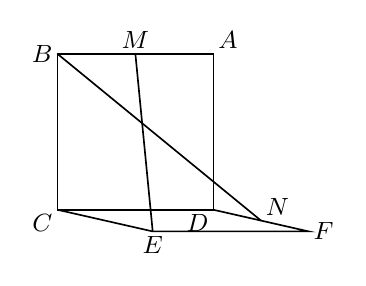
\begin{tikzpicture}[scale=1.1, semithick, every node/.style={inner sep=1.5pt, font=\small}]
  \coordinate (D) at (0,0);
  \coordinate (C) at (-1.8,0);
  \coordinate (B) at (-1.8,1.8);
  \coordinate (A) at (0,1.8);
  \coordinate (E) at (-0.7,-0.25);
  \coordinate (F) at (1.1,-0.25);
  \coordinate (M) at (-0.9,1.8);
  \coordinate (N) at (0.55,-0.125);
  % 竖直正方形 ABCD
  \draw (A) -- (B) -- (C) -- (D) -- cycle;
  % 水平正方形 DCEF
  \draw (C) -- (E) -- (F) -- (D);
  % 图中线段 ME、BN
  \draw (M) -- (E);
  \draw (B) -- (N);
  % 顶点标注
  \node[above right] at (A) {$A$};
  \node[left] at (B) {$B$};
  \node[above] at (M) {$M$};
  \node[below left] at (C) {$C$};
  \node[below left] at (D) {$D$};
  \node[below] at (E) {$E$};
  \node[right] at (F) {$F$};
  \node[above right] at (N) {$N$};
\end{tikzpicture}
\end{center}
\nopagebreak[4]
\end{question}
\begin{question}
\gkti{19}某人向一目射击 $4$ 次，每次击中目标的概率为 $\frac13$．该目标分为 $3$ 个不同的部分，第一、二、三部分面积之比为 $1:3:6$．击中目标时，击中任何一部分的概率与其面积成正比．

（1）设 $X$ 表示目标被击中的次数，求 $X$ 的分布列；

（2）若目标被击中 $2$ 次，$A$ 表示事件“第一部分至少被击中 $1$ 次或第二部分被击中 $2$ 次”，求 $P(A)$．

\end{question}
\begin{question}
\gkti{20}已知椭圆 $C$ 过点 $A\left(1,\frac32\right)$，两个焦点为 $(-1,0)$，$(1,0)$．

（1）求椭圆 $C$ 的方程；

（2）$E,F$ 是椭圆 $C$ 上的两个动点，如果直线 $AE$ 的斜率与 $AF$ 的斜率互为相反数，证明直线 $EF$ 的斜率为定值，并求出这个定值．

\end{question}
\begin{question}
\gkti{21}已知函数 $f(x)=\frac12x^2-ax+(a-1)\ln x$，$a>1$．

（1）讨论函数 $f(x)$ 的单调性；

\Needspace{5\baselineskip}
（2）证明：若 $a<5$，则对于任意 $x_1,x_2\in(0,+\infty)$，$x_1\neq x_2$，有

\nopagebreak[4]
\[\frac{f(x_1)-f(x_2)}{x_1-x_2}>-1 .\]

\Needspace{0.4\textheight}
\end{question}
\begin{question}
\gkti{22}三选一．

\textbf{【A】} 已知 $\triangle ABC$ 中，$AB=AC$，$D$ 是 $\triangle ABC$ 外接圆劣弧 $\overset{\frown}{AC}$ 上的点（不与点 $A,C$ 重合），延长 $BD$ 至 $E$．

（1）求证：$AD$ 的延长线平分 $\angle CDE$；

（2）若 $\angle BAC=30^\circ$，$\triangle ABC$ 中 $BC$ 边上的高为 $2+\sqrt3$，求 $\triangle ABC$ 外接圆的面积．

\textbf{【B】} 在直角坐标系 $xOy$ 中，以 $O$ 为极点，$x$ 正半轴为极轴建立极坐标系，曲线 $C$ 的极坐标方程为 $\rho\cos\left(\theta-\frac{\pi}{3}\right)=1$，$M,N$ 分别为 $C$ 与 $x$ 轴、$y$ 轴的交点．

（1）写出 $C$ 的直角坐标方程，并求 $M,N$ 的极坐标；

（2）设 $MN$ 的中点为 $P$，求直线 $OP$ 的极坐标方程．

\textbf{【C】} 设函数 $f(x)=|x-1|+|x-a|$．

（1）若 $a=-1$，解不等式 $f(x)\geqslant3$；

（2）如果 $\forall x\in\mathbf R$，$f(x)\geqslant2$，求 $a$ 的取值范围．
\nopagebreak[4]
\begin{center}% 2009 年辽宁卷理科第 22 题【A】：△ABC 的外接圆，D 是劣弧 AC 上的点，延长 BD 至 E。
% 来源 PDF：普通高考/2009/2009辽宁理.pdf，SHA256 5ae9708acfe7def5bddd60a34d1474cfa2e2c20a39d130255e0e4393093accad
% 原页：第 2 页（A3 三栏）第 3 栏上部，印刷页 538。
% 重绘依据：A 在圆上最高处，B、C 在下方左右对称（AB=AC），D 在 A 与 C 之间的劣弧上，
%   B、D、E 共线且 E 在 D 的延长线上；连 AB、AC、AD、BC、CD，并延长 BD 至 E。
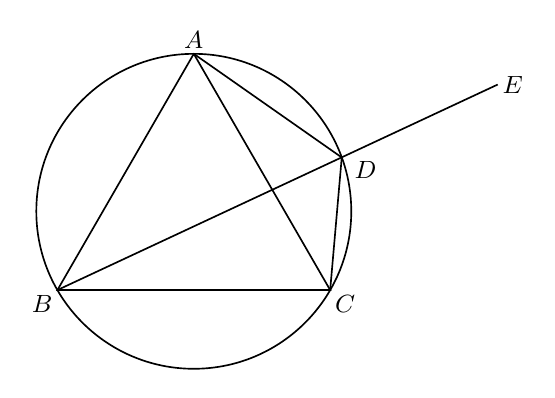
\begin{tikzpicture}[scale=1.0, semithick, every node/.style={inner sep=1.5pt, font=\small}]
  \coordinate (O) at (0,0);
  \coordinate (A) at (0,2);
  \coordinate (B) at (-1.732,-1);
  \coordinate (C) at (1.732,-1);
  \coordinate (D) at (1.879,0.684);
  \coordinate (E) at (3.86,1.61);
  % 外接圆
  \draw (O) circle (2);
  % 三角形与相关线段
  \draw (A) -- (B) -- (C) -- (A);
  \draw (A) -- (D);
  \draw (C) -- (D);
  \draw (B) -- (E);
  % 顶点标注
  \node[above] at (A) {$A$};
  \node[below left] at (B) {$B$};
  \node[below right] at (C) {$C$};
  \node[right] at (1.98,0.52) {$D$};
  \node[right] at (E) {$E$};
\end{tikzpicture}
\end{center}
\nopagebreak[4]

\end{question}